\section{Methodology}
\label{sec:methodology}
In this section, the methodology proposed in this study is presented. Firstly, approach overview is described from a high-level perspective. Then, each stage in the methodology is presented together with their importance in the study, mathematical representations and definitions; and black-box diagrams. In the last section of this chapter, implementation details of this methodology in ProM framework is explained in detail with a software architecture overview.

\subsection{Approach Overview}
\label{subsec:approach-overview}
The approach proposed in this study consists of four main stages visualized in Figure~\ref{fig:approach-overview}. Firstly, in \textit{Process Model Mining}, process models are extracted from event logs for each organization with a user specified noise threshold. Secondly, in \textit{Performance Indicator Analysis}, event logs are replayed on process models and performance indicators are calculated for each organization then using these indicators, organizations are clustered based on how well they are operating. Thirdly, in \textit{Mismatch Pattern Analysis}, differences between process models of organizations are extracted with well-established mismatch patterns. Finally, in \textit{Recommendation Generation}, using the performance indicator clusterings and differences between process models, a set of recommendations for each organization is generated. In the following sections, each stage will be explained in detail with their mathematical backgrounds.

\begin{figure}
  \centering
  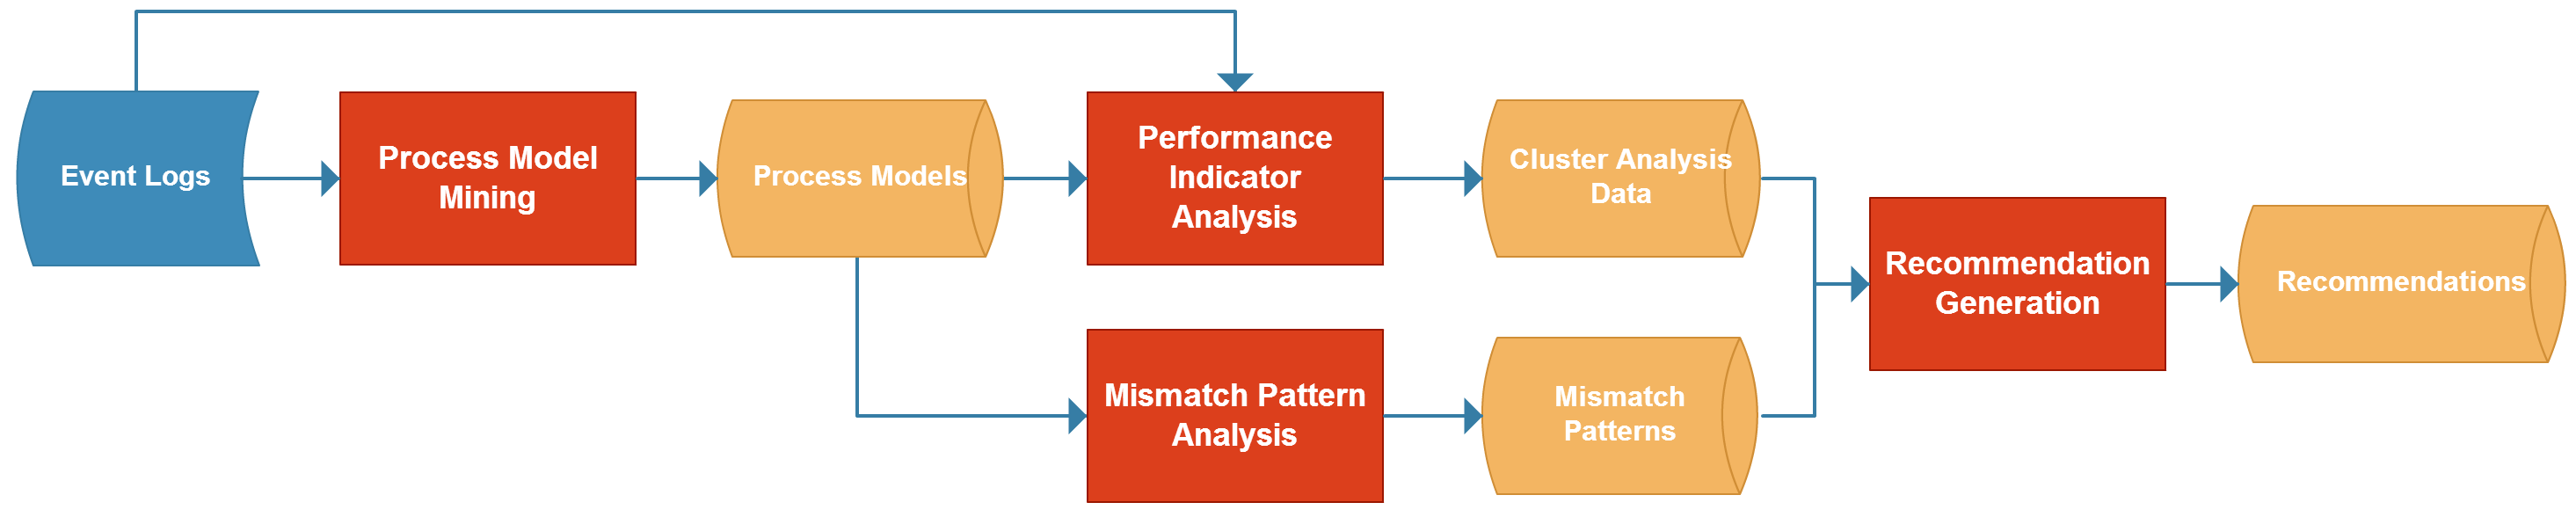
\includegraphics[width=\textwidth]{4_methodology/approach-overview}
  \caption{Overview of Methodology}
  \label{fig:approach-overview}
\end{figure}

\subsection{Process Model Mining}
\label{subsec:process-model-mining}
Process model mining in the proposed approach has the aim of creating reproducible and generalized process models from event logs. In order to achieve this aim, implementation of \textit{Inductive Miner Infrequent (IMi)}, which is proposed in \cite{leemans2014discoveringinfrequent} as an extension to \textit{Inductive Miner} to handle noise in the event logs, is used in this study. Considering the scope of this study, instead of computational details of \textit{Inductive Miner Infrequent (IMi)}; black-box representation is used to explain its usage in the methodology. In order to set a filtering threshold, a user-provided value between 0 to 1 is added as input to method in addition to event logs. As a result, workflow net is produced which is a sound and properly completed Petri net without deadlocks. Black-box of this stage is illustrated in Figure~\ref{fig:process-model-mining-blackbox} and this stage is called for every organization's event logs to create their own process models in Workflow net formalization.

\begin{figure}
  \centering
  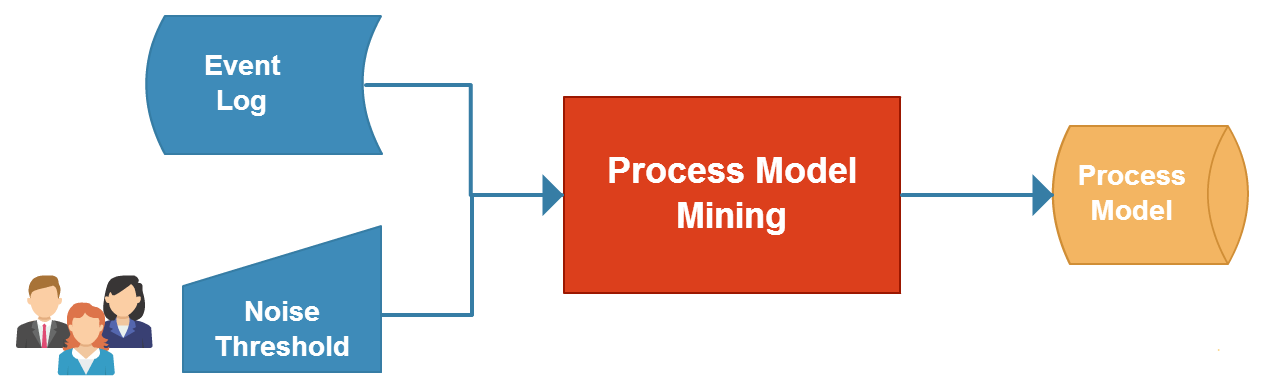
\includegraphics[width=0.5\textwidth]{4_methodology/process-model-mining-blackbox}
  \caption{Process Model Mining Stage as Black-box }
  \label{fig:process-model-mining-blackbox}
\end{figure}

\subsection{Performance Indicator Analysis}
\label{subsec:performance-indicator-analysis}
Performance indicator analysis stage focuses on calculating and analyzing the performance values using the event logs and mined process models. This stage consists of mainly two concepts as 
\begin{inparaenum}[\itshape a\upshape)]
\item alignment and calculation of performance indicators; and
\item clustering of organizations based on their performance values.
\end{inparaenum}
In order to evaluate the performance of an organization based on their process models and past activities; there is a number of indicators in time dimension, cost dimension and utilization \cite{van2011process}. However, in this study, process related performance values are considered since differences in the process models are studied in the next stages. With this reasoning, the following performance indicators are calculated and analyzed in this stage of methodology:
\begin{description}
	\item[Average Time Between Activities] For each activity in the process model, average time to reach other activity is calculated. This is a simple but powerful performance metric for organizations since it can yield the average time to complete one task based on a starting point. From the performance perspective, organizations want to minimize average time between activities to increase their throughput \cite{van2012replaying}.
	\item[Standard Deviation of Time Between Activities] Time between activities in real life is not stable and they deviate due to various reasons such as people responsible of tasks, size and the content of tasks or seasonality \cite{van2011process}. On the other hand, organizations want to be confident about their processes and therefore they want to minimize the deviation in the time between activities. Minimized deviation in time helps organizations to plan, act and re-organize the activities in the processes with high accuracy \cite{van2012replaying}. 
\end{description}

\subsubsection{Replay and Performance Indicator Calculation}
\label{subsubsec:replay-and-performance-summary}
Replay of event logs on process models is based on the idea of \textit{alignment} which is formalized in \cite{van2012replaying} and the basic assumption in this concept is that process models and event logs have the same activity labels. Alignment is based on \textit{moves in the model and log} and in order to have a successful replay where optimal alignment should be achieved. As proposed in \cite{adriansyah2011conformance, adriansyah2011towards}, $A^{*}$ algorithm which is a path-finding algorithm based on graphs is used to find optimal alignment of event logs on the process models. With the generated and user-specified inputs, replay and performance indicator calculation in the methodology can be visualized in Figure~\ref{fig:replay-and-performance-indicator-calculation}. For each organization, the steps in the diagram are followed with the corresponding event logs and process models; and the resulting process summaries are used for further analysis.

\begin{figure}
  \centering
  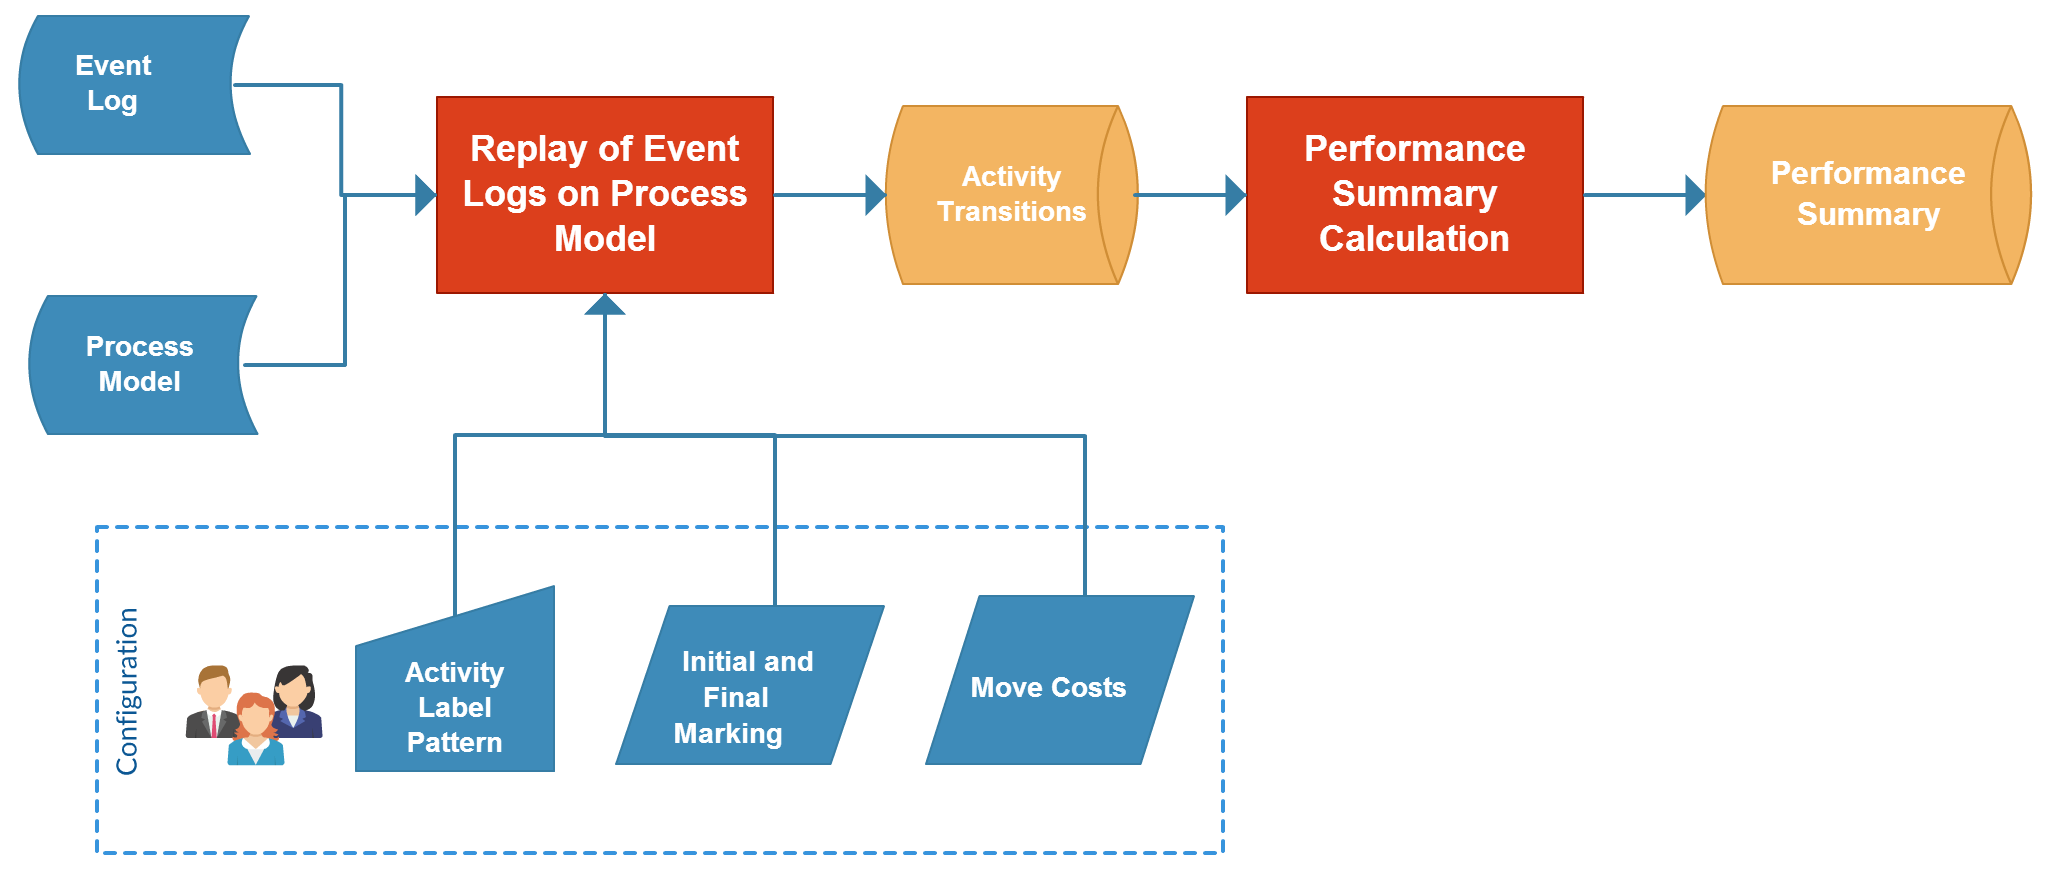
\includegraphics[width=\textwidth]{4_methodology/replay-and-performance-indicator-calculation}
  \caption{Replay and Performance Indicator Calculation Stage as Black-box}
  \label{fig:replay-and-performance-indicator-calculation}
\end{figure}

\subsubsection{Performance Indicator Clustering}
\label{subsubsec:performance-indicator-clustering}

Clustering is based on the idea of collecting the set of observations into clusters so that observations within the same cluster are similar whereas the observations from different clusters are dissimilar. In this thesis study, clustering is used to gather organizations based on their performance indicator data. In this study, a generic approach based on centroid-based clustering is exploited. For the fixed number of \textit{k} clusters, the approach is well-known as \textit{k-means clustering}. Considering the popularity of this approach and its extensions, random initialization based \textit{k-means++} approach from the study of Arthur and Vassilvitskii \cite{arthur2007} is used to cluster organizations. For each organization, \textit{Performance Summary} data is used as the data source in clustering. Since number of clusters are not known priori, k-means clustering is applied starting \textit{k} from 1 to the number of organizations. For each clustering with different number of clusters, SSE values are plotted and user is made to select the appropriate cluster size. For the selected cluster size, clustering related information is used to generate recommendations in the further steps. This stage of methodology can be visualized as an input-output system in Figure~\ref{fig:performance-indicator-clustering-blackbox}. 
\begin{figure}
  \centering
  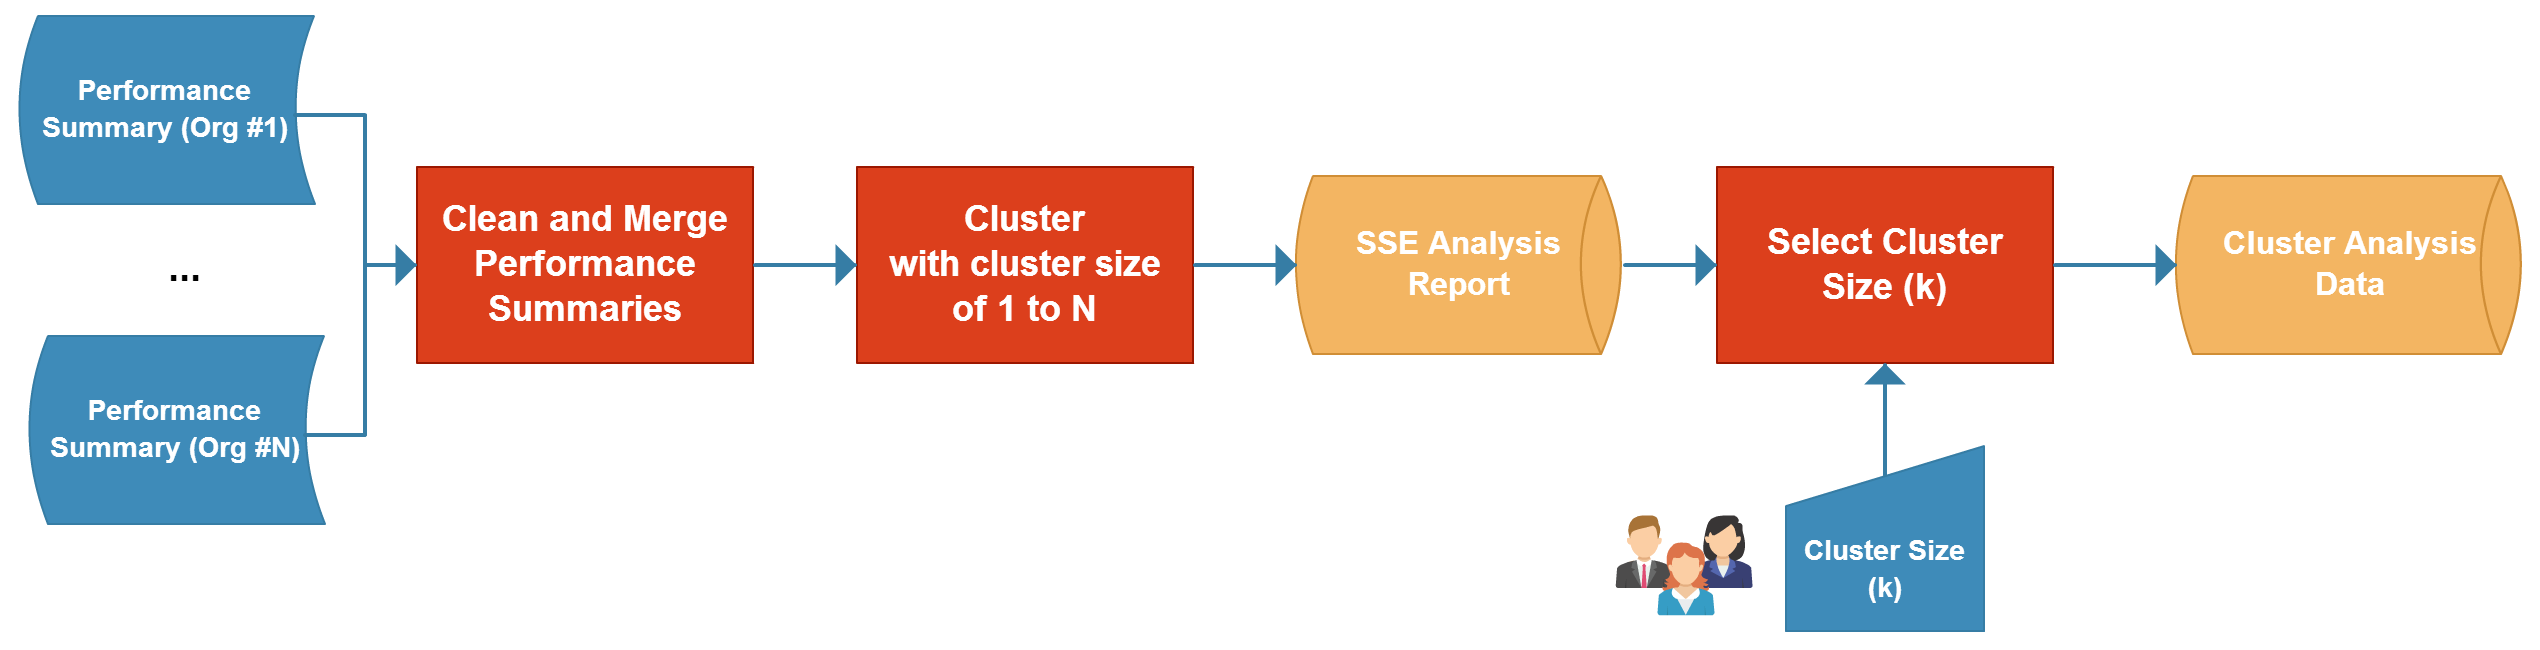
\includegraphics[width=\textwidth]{4_methodology/performance-indicator-clustering-blackbox}
  \caption{Performance Indicator Clustering Stage as Black-box }
  \label{fig:performance-indicator-clustering-blackbox}
\end{figure}